\documentclass[]{beamer}\makeatletter

\IfFileExists{xcolor.sty}%
  {\RequirePackage{xcolor}}%
  {\RequirePackage{color}}
\usepackage{colortbl}
      
\usepackage{fontspec}
\usepackage{xunicode}
\catcode`⃥=\active \def⃥{\textbackslash}
\catcode`❴=\active \def❴{\{}
\catcode`❵=\active \def❵{\}}
\def\textJapanese{\fontspec{Kochi Mincho}}
\def\textChinese{\fontspec{HAN NOM A}\XeTeXlinebreaklocale "zh"\XeTeXlinebreakskip = 0pt plus 1pt }
\def\textKorean{\fontspec{Baekmuk Gulim} }
\setmonofont{DejaVu Sans Mono}

\DeclareTextSymbol{\textpi}{OML}{25}
\usepackage{relsize}
\def\textsubscript#1{%
  \@textsubscript{\selectfont#1}}
\def\@textsubscript#1{%
  {\m@th\ensuremath{_{\mbox{\fontsize\sf@size\z@#1}}}}}
\def\textquoted#1{‘#1’}
\def\textsmall#1{{\small #1}}
\def\textlarge#1{{\large #1}}
\def\textoverbar#1{\ensuremath{\overline{#1}}}
\def\textgothic#1{{\fontspec{Lucida Blackletter}#1}}
\def\textcal#1{{\fontspec{Lucida Calligraphy}#1}}
\RequirePackage{array}
\def\@testpach{\@chclass
 \ifnum \@lastchclass=6 \@ne \@chnum \@ne \else
  \ifnum \@lastchclass=7 5 \else
   \ifnum \@lastchclass=8 \tw@ \else
    \ifnum \@lastchclass=9 \thr@@
   \else \z@
   \ifnum \@lastchclass = 10 \else
   \edef\@nextchar{\expandafter\string\@nextchar}%
   \@chnum
   \if \@nextchar c\z@ \else
    \if \@nextchar l\@ne \else
     \if \@nextchar r\tw@ \else
   \z@ \@chclass
   \if\@nextchar |\@ne \else
    \if \@nextchar !6 \else
     \if \@nextchar @7 \else
      \if \@nextchar (8 \else
       \if \@nextchar )9 \else
  10
  \@chnum
  \if \@nextchar m\thr@@\else
   \if \@nextchar p4 \else
    \if \@nextchar b5 \else
   \z@ \@chclass \z@ \@preamerr \z@ \fi \fi \fi \fi
   \fi \fi  \fi  \fi  \fi  \fi  \fi \fi \fi \fi \fi \fi}

\gdef\arraybackslash{\let\\=\@arraycr}
\def\textxi{\ensuremath{\xi}}
\def\Panel#1#2#3#4{\multicolumn{#3}{){\columncolor{#2}}#4}{#1}}

\newcolumntype{L}[1]{){\raggedright\arraybackslash}p{#1}}
\newcolumntype{C}[1]{){\centering\arraybackslash}p{#1}}
\newcolumntype{R}[1]{){\raggedleft\arraybackslash}p{#1}}
\newcolumntype{P}[1]{){\arraybackslash}p{#1}}
\newcolumntype{B}[1]{){\arraybackslash}b{#1}}
\newcolumntype{M}[1]{){\arraybackslash}m{#1}}
\definecolor{label}{gray}{0.75}
\DeclareRobustCommand*{\xref}{\hyper@normalise\xref@}
\def\xref@#1#2{\hyper@linkurl{#2}{#1}}
\def\Div[#1]#2{\section*{#2}}
\begingroup
\catcode`\_=\active
\gdef_#1{\ensuremath{\sb{\mathrm{#1}}}}
\endgroup
\mathcode`\_=\string"8000
\catcode`\_=12\relax

\usepackage{framed}
\usepackage{fontspec}
\usepackage{colortbl}
\usepackage{xunicode}
%\setmonofont{Junicode}
%\setmonofont[Scale=0.86]{Lucida Sans Typewriter}
%\setmonofont[Scale=0.86]{Andale Mono}
\setmonofont[Scale=0.8]{DejaVu Sans Mono}
\setromanfont{Minion Pro}
\setsansfont{Myriad Pro}
\usetheme{Singapore}
\useinnertheme[shadow=true]{rounded}
\usecolortheme{orchid}
\setbeamercolor*{frametitle}{parent=palette primary}
\definecolor{shadecolor}{gray}{0.875}
\usepackage{fancyvrb,fancyhdr,longtable}
\def\Gin@extensions{.pdf,.png,.jpg,.mps,.tif}
\setbeamercovered{transparent}
\usenavigationsymbolstemplate{}
\xdefinecolor{blue1}{rgb}{0, 0, 0.7}
\xdefinecolor{blue2}{rgb}{0, 0, 1}
\let\mainmatter\relax
\let\frontmatter\relax
\let\backmatter\relax
\let\endfoot\relax
\let\endlastfoot\relax
\parskip3pt
\setbeamertemplate{footline}
{\hspace{1em}
\includegraphics[height=4ex]{logo.png} \hspace{2em}
\hfill \textcolor{gray}{\insertframenumber/\inserttotalframenumber}
\vspace{1em}}

\date{}
\institute{}
\pgfdeclareimage[height=1cm]{logo}{../Graphics/logo}
\logo{\pgfuseimage{logo}}

\@ifundefined{chapter}{%
    \def\DivI{\section}
    \def\DivII{\subsection}
    \def\DivIII{\subsubsection}
    \def\DivIV{\paragraph}
    \def\DivV{\subparagraph}
    \def\DivIStar[#1]#2{\section*{#2}}
    \def\DivIIStar[#1]#2{\subsection*{#2}}
    \def\DivIIIStar[#1]#2{\subsubsection*{#2}}
    \def\DivIVStar[#1]#2{\paragraph*{#2}}
    \def\DivVStar[#1]#2{\subparagraph*{#2}}
}{%
    \def\DivI{\chapter}
    \def\DivII{\section}
    \def\DivIII{\subsection}
    \def\DivIV{\subsubsection}
    \def\DivV{\paragraph}
    \def\DivIStar[#1]#2{\chapter*{#2}}
    \def\DivIIStar[#1]#2{\section*{#2}}
    \def\DivIIIStar[#1]#2{\subsection*{#2}}
    \def\DivIVStar[#1]#2{\subsubsection*{#2}}
    \def\DivVStar[#1]#2{\paragraph*{#2}}
}
\def\TheFullDate{2010-11 (revised: 
    2010-11)}
\def\TheID{\makeatother }
\def\TheDate{2010-11}
\title{Encodage des textes     patrimoniaux {\hskip1pt}\newline Le manuscrit (1)      Transcription}
\author{Lou Burnard}\let\tabcellsep&
      \catcode`\&=12\relax \makeatletter \makeatother 
\begin{document}

     \frame{\maketitle}
   
\catcode`\$=12\relax
\catcode`\^=12\relax
\catcode`\#=12\relax
\catcode`\%=12\relax

\begin{frame}
\frametitle{Objectifs}\begin{itemize}

\item découvrir les balises spécifiques pour l’encodage de       transcriptions des manuscrits
\item lettres, abbreviations, ratures, choice, etc,
\item faire le point sur l'édition génétique
\item facsimilé, liens image/transcription 
\end{itemize} 
\end{frame}

\begin{frame}
\frametitle{La transcription des sources primaires}\par
Quelles caractéristiques d’une source primaire pourrait-on vouloir      exprimer dans un travail de transcription ? \begin{itemize}

\item la manière dont le texte est inscrit sur la page
\item l’orthographe
\item le rendu formel original (s’il a une importance)
\item la ponctuation originale
\item les abréviations
\item les ajouts et suppressions
\item les erreurs et omissions
\item  eventuellement, les illustrations, dessins ou graphiques       illustrant le texte
\item la structure logique du texte
\item peut-être d’autres choses, selon le point de vue qu’on adopte et       les objectifs du projet...
\end{itemize} 
\end{frame}

\begin{frame}
\frametitle{Objectifs d'un projet de transcription}\begin{itemize}

\item mettre à disposition du plus grand nombre de chercheurs -- ou       curieux -- des sources primaires
\item ... en les rendant compréhensibles à un public moderne
\item établir un texte definitif à partir de plusieurs témoins,       completer la transcription avec un stemma ou tableau de la       tradition, et des notes d’apparat critique
\item mettre en place un paratexte fournissant des notes explicatives       ou historiques pour identifier un lieu, une personne, etc.
\end{itemize} \par\begin{exampleblock}{}
Dans tous les cas, la transcription devrait s'appuyer sur      des règles éditoriales qui seront explicitées, et qui seront      elles-mêmes fondées sur des recommandations admises dans la discipline      scientifique concernée.\end{exampleblock}\par

\end{frame}

\begin{frame}
\frametitle{Les principaux éléments TEI utiles pour la transcription}\begin{description}

\item[Définis dans le module 'core' :]{\color{blue2}<abbr>}, {\color{blue2}<add>}, {\color{blue2}<choice>}, {\color{blue2}<corr>},        {\color{blue2}<del>}, {\color{blue2}<expan>}, {\color{blue2}<gap>}, {\color{blue2}<sic>}
\item[Définis dans le module 'transcr' :]{\color{blue2}<addSpan>}, {\color{blue2}<am>}, {\color{blue2}<damage>}, {\color{blue2}<damageSpan>},        {\color{blue2}<delSpan>}, {\color{blue2}<ex>}, {\color{blue2}<facsimile>}, {\color{blue2}<fw>},        {\color{blue2}<handNotes>}, {\color{blue2}<handShift>}, {\color{blue2}<restore>}{\color{blue2}<space>}, {\color{blue2}<subst>}, {\color{blue2}<supplied>}, {\color{blue2}<surface>},        {\color{blue2}<zone>}
\item[Définis dans le module 'textcrit' :]{\color{blue2}<app>}, {\color{blue2}<lacunaEnd>}, {\color{blue2}<lacunaStart>},       {\color{blue2}<lem>}, {\color{blue2}<listWit>}, {\color{blue2}<rdg>}, {\color{blue2}<rdgGrp>},        {\color{blue2}<variantEncoding>}, {\color{blue2}<wit>}, {\color{blue2}<witDetail>},        {\color{blue2}<witEnd>}, {\color{blue2}<witStart>}, {\color{blue2}<witness>}
\end{description} 
\end{frame}

\begin{frame}
\frametitle{Structure logique et mise en page du texte}\par
Par \textit{structure}, on entend l’organisation du texte en      parties constituantes, par \textit{mise en page} la manière dont      le texte est inscrit, réparti, sur le support.\par
Le texte étudié et l’objet physique sur lequel ce texte est inscrit      ont des structures hiérarchiques distinctes, qu’il faut toutes les      deux encoder dans l’idéal... \par
... ce qui provoque des problemes de chevauchement.\par\begin{exampleblock}{}
Pour la structure logique, les manuscrits et les imprimes      ont tous les deux les memes possibilites. \end{exampleblock}\par

\end{frame}

\begin{frame}
\frametitle{Encodage de la structure physique}\par
Pour exprimer la manière dont le texte est inscrit sur le support      physique, des éléments vides de type ‘milestone’      (borne) sont disponibles, {\color{blue2}<gb/>}, {\color{blue2}<pb/>}, {\color{blue2}<cb/>}, et       {\color{blue2}<lb/>}, qui correspondent respectivement à la désignation des      debuts de cahier ("gathering"), page, colonne et ligne. \par
Comme tout élément, on peut numéroter et identifier ceux-ci au moyen      des attributs \emph{@n} et \emph{@xml:id} pour etablir un      systeme de referencement.
\end{frame}

\begin{frame}
\frametitle{Encodage de la structure physique : exemple}\par
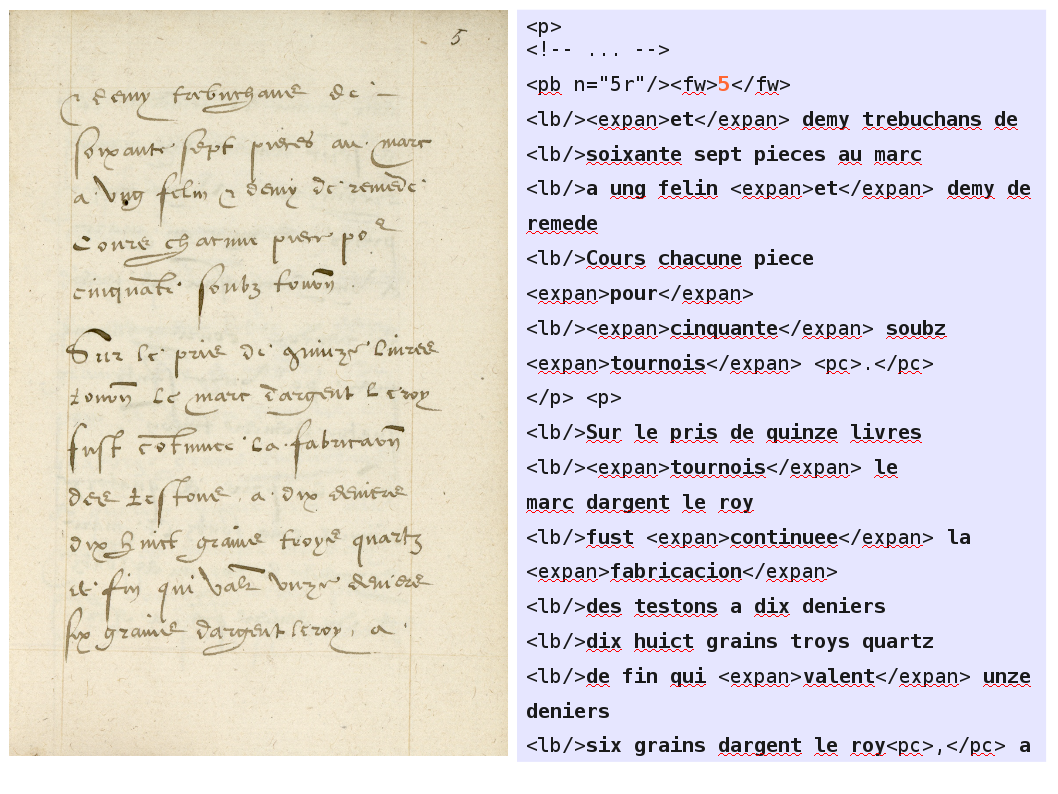
\includegraphics[width=\textwidth]{../Graphics/exemple-p5.png}  
\end{frame}

\begin{frame}[fragile]
\frametitle{Titres courants, réclames, etc.}\begin{description}

\item[{\color{blue2}<fw>}]L’élément {\color{blue2}<fw>} (forme work, ou élément de mise en page)       permet d’encoder un titre courant (en haut ou en bas de la page),       une réclame ou une autre information comparable, qui apparaît sur la       page courante.
\end{description} 
\bgroup\ttfamily\fontsize{8.5pt}{9pt}\selectfont\par
\begin{exampleblock}{}
\noindent\ttfamily\mbox{}{\color{blue1}<\textbf{fw}\hspace*{6pt}place="{\color{blue2}top-centre}"\hspace*{6pt}type="{\color{blue2}head}">}Poëms.{\color{blue1}</\textbf{fw}>}\mbox{}\newline 
{\color{blue1}<\textbf{fw}\hspace*{6pt}place="{\color{blue2}top-right}"\hspace*{6pt}type="{\color{blue2}pageno}">}29{\color{blue1}</\textbf{fw}>}\mbox{}\newline 
{\color{blue1}<\textbf{fw}\hspace*{6pt}place="{\color{blue2}bot-centre}"\hspace*{6pt}type="{\color{blue2}sig}">}E3{\color{blue1}</\textbf{fw}>}\mbox{}\newline 
{\color{blue1}<\textbf{fw}\hspace*{6pt}place="{\color{blue2}bot-right}"\hspace*{6pt}type="{\color{blue2}catch}">}TEMPLE{\color{blue1}</\textbf{fw}>}
\end{exampleblock}
\par\egroup
  \par\begin{exampleblock}{}
Nota: cet élément sert à encoder les references déjà existant dans le manuscrit.\end{exampleblock}\par

\end{frame}

\begin{frame}
\frametitle{Les abréviations}\par
Les abréviations sont très caractéristiques des manuscrits de toutes      sortes. On distingue plusieurs types d’abréviations :       \begin{description}

\item[Abréviations par suspension]la ou les premières lettres du mot sont écrites, suivies en        général d’un point ou d’une autre marque : par exemple ‘e.g.’        pour ‘exempli gratia’. 
\item[Abréviations par contraction]les première(s) et dernière(s) lettres du mot sont écrites,        accompagnées le plus souvent d’un signe abréviatif tel que trait        suscrit, ou, plus rarement, un point : par exemple ‘ā’ pour        ‘an’, ‘M.’ pour         ‘Monsieur’ etc. 
\item["Brévigraphes"]ce sont des symboles spécifiques, tels que la note tironienne        (&#x204A; ⁊) utilisée à la place de la conjonction de coordination         ‘et’, la lettre p barrée (&#x1D71; ᵱ), souvent utilisée à        la place de la syllabe ‘per’. 
\end{description}      \par
La plupart des symboles dont on a besoin sont définies par Unicode, mais ne sont pas forcément presente dans toutes les polices.
\end{frame}

\begin{frame}
\frametitle{Les abréviations et leur résolution}\par
Une abréviation peut être restituée de deux manières : \begin{itemize}

\item on peut choisir de consigner l’abréviation non développée, en        la transcrivant simplement tel quel: par exemple, ‘po suivi de r        superieure’ ou un ‘a avec macron’
\item on peut aussi interpréter ou développer l’abréviation, en        remplaçant la ou les lettres par leur signification : par exemple,        ‘pour’, ‘an’
\end{itemize}      \par
La TEI permet de fournir à la fois les formes abrégées et développées      des abréviations.
\end{frame}

\begin{frame}
\frametitle{Encoder les abréviations}\par
La TEI propose deux niveaux d’encodage : \begin{itemize}

\item la totalité d’un mot abrégé et la totalité de sa forme        développée peuvent être encodés au moyen des éléments         {\color{blue2}<abbr>} et {\color{blue2}<expan>}
\item le symbole utilisé pour indiquer la suppression d’une ou        plusieurs lettres peut etre encodé par l'élément {\color{blue2}<am>}; les        lettres substituées à ce symbole lorsqu’on résoud l’abréviation        par l'élément {\color{blue2}<ex>}
\end{itemize} Ici aussi on peut utiliser les deux niveaux conjointement.
\end{frame}

\begin{frame}[fragile]
\frametitle{Un exemple}\par

\includegraphics[width=360pt,]{../Graphics/Ms629_p05-dtl-1.png}. \par
Selon la stratégie éditoriale, on peut signaler simplement qu'il y      avait des formes abrégés qu'on a rétablis: 
\bgroup\ttfamily\fontsize{8.5pt}{9pt}\selectfont\par
\begin{exampleblock}{}
\noindent\ttfamily\mbox{}{\color{blue1}<\textbf{p}>}\mbox{}\newline 
\hspace*{6pt}{\color{blue1}<\textbf{lb}/>}Cours chacune piece {\color{blue1}<\textbf{expan}>}pour{\color{blue1}</\textbf{expan}>}\mbox{}\newline 
\hspace*{6pt}{\color{blue1}<\textbf{lb}/>}\mbox{}\newline 
\hspace*{6pt}{\color{blue1}<\textbf{expan}>}cinquante{\color{blue1}</\textbf{expan}>} soubz\mbox{}\newline 
{\color{blue1}<\textbf{expan}>}tournois{\color{blue1}</\textbf{expan}>}\mbox{}\newline 
\hspace*{6pt}{\color{blue1}<\textbf{pc}>}.{\color{blue1}</\textbf{pc}>}\mbox{}\newline 
{\color{blue1}</\textbf{p}>}
\end{exampleblock}
\par\egroup
  
\end{frame}

\begin{frame}[fragile]
\frametitle{Encodage des formes graphiques des abbreviations}\par
Mais, en effet, ‘pour’ a ete ecrit ‘po’ suivi d'une  lettre ‘r’ suscrite; ‘cinquante’ comme ‘cinquāte’      avec un macron sur le ‘a’ pour signaler la nasalisation. \par
On pourrait donc encoder ces mots de l’une ou l’autre des manières      ci-après  : 
\bgroup\ttfamily\fontsize{8.5pt}{9pt}\selectfont\par
\begin{exampleblock}{}
\noindent\ttfamily\mbox{}{\color{blue1}<\textbf{p}>}\mbox{}\newline 
\hspace*{6pt}{\color{blue1}<\textbf{abbr}>}po&#xFFFD;{\color{blue1}</\textbf{abbr}>} .... {\color{blue1}<\textbf{abbr}>}cinquāte{\color{blue1}</\textbf{abbr}>}\mbox{}\newline 
{\color{blue1}</\textbf{p}>}
\end{exampleblock}
\par\egroup
       \par
... ou : 
\bgroup\ttfamily\fontsize{8.5pt}{9pt}\selectfont\par
\begin{exampleblock}{}
\noindent\ttfamily\mbox{}{\color{blue1}<\textbf{p}>} po{\color{blue1}<\textbf{am}>}&#xFFFD;{\color{blue1}</\textbf{am}>} ... ou po{\color{blue1}<\textbf{ex}>}u{\color{blue1}</\textbf{ex}>}r {\color{blue1}</\textbf{p}>}
\end{exampleblock}
\par\egroup
        
\bgroup\ttfamily\fontsize{8.5pt}{9pt}\selectfont\par
\begin{exampleblock}{}
\noindent\ttfamily\mbox{}{\color{blue1}<\textbf{p}>}\mbox{}\newline 
\hspace*{6pt}{\color{blue1}<\textbf{abbr}>}po{\color{blue1}<\textbf{am}>}&#xFFFD;{\color{blue1}</\textbf{am}>}\mbox{}\newline 
\hspace*{6pt}{\color{blue1}</\textbf{abbr}>} ou\mbox{}\newline 
{\color{blue1}<\textbf{expan}>}po{\color{blue1}<\textbf{ex}>}u{\color{blue1}</\textbf{ex}>}r{\color{blue1}</\textbf{expan}>}\mbox{}\newline 
{\color{blue1}</\textbf{p}>}
\end{exampleblock}
\par\egroup
       
\end{frame}

\begin{frame}[fragile]
\frametitle{Utilisation de {\color{blue2}<choice>}}\par
Toutes ces paires d’éléments peuvent être englobées dans un élément       {\color{blue2}<choice>} (choix) : 
\bgroup\ttfamily\fontsize{8.5pt}{9pt}\selectfont\par
\begin{exampleblock}{}
\noindent\ttfamily\mbox{}{\color{blue1}<\textbf{p}>} po{\color{blue1}<\textbf{choice}>}\mbox{}\newline 
\hspace*{6pt}\hspace*{6pt}{\color{blue1}<\textbf{am}>}&#FFFD;{\color{blue1}</\textbf{am}>}\mbox{}\newline 
\hspace*{6pt}\hspace*{6pt}{\color{blue1}<\textbf{ex}>}ur{\color{blue1}</\textbf{ex}>}\mbox{}\newline 
\hspace*{6pt}{\color{blue1}</\textbf{choice}>}\mbox{}\newline 
{\color{blue1}</\textbf{p}>}
\end{exampleblock}
\par\egroup
        
\bgroup\ttfamily\fontsize{8.5pt}{9pt}\selectfont\par
\begin{exampleblock}{}
\noindent\ttfamily\mbox{}{\color{blue1}<\textbf{choice}>}\mbox{}\newline 
\hspace*{6pt}{\color{blue1}<\textbf{abbr}>}po{\color{blue1}<\textbf{am}>}&#xFFFD;{\color{blue1}</\textbf{am}>}\mbox{}\newline 
\hspace*{6pt}{\color{blue1}</\textbf{abbr}>}\mbox{}\newline 
\hspace*{6pt}{\color{blue1}<\textbf{expan}>}po{\color{blue1}<\textbf{ex}>}u{\color{blue1}</\textbf{ex}>}r{\color{blue1}</\textbf{expan}>}\mbox{}\newline 
{\color{blue1}</\textbf{choice}>}
\end{exampleblock}
\par\egroup
       
\end{frame}

\begin{frame}[fragile]
\frametitle{Catégoriser les abréviations}\par
L’attribut \emph{@type} de l’élément {\color{blue2}<abbr>} sert a      catégoriser les abréviations, qu’il s’agisse de préparer une analyse      statistique ou de restituer ces abréviations de manière différente      selon leur type. \par
Par exemple, on peut vouloir afficher le développement des      abréviations par suspension entre crochets, d’autres types en italique      ou entre parenthèses etc. 
\bgroup\ttfamily\fontsize{8.5pt}{9pt}\selectfont\par
\begin{exampleblock}{}
\noindent\ttfamily\mbox{}{\color{blue1}<\textbf{choice}>}\mbox{}\newline 
\hspace*{6pt}{\color{blue1}<\textbf{abbr}\hspace*{6pt}type="{\color{blue2}brevigraphe}">}po{\color{blue1}<\textbf{am}>}&#xFFFD;{\color{blue1}</\textbf{am}>}\mbox{}\newline 
\hspace*{6pt}{\color{blue1}</\textbf{abbr}>}\mbox{}\newline 
\hspace*{6pt}{\color{blue1}<\textbf{expan}>}po{\color{blue1}<\textbf{ex}>}u{\color{blue1}</\textbf{ex}>}r{\color{blue1}</\textbf{expan}>}\mbox{}\newline 
{\color{blue1}</\textbf{choice}>}
\end{exampleblock}
\par\egroup
   L'inscription encodée ci-dessus peut être affichée comme      suit : ‘po(u)r’     \par
Comme ailleurs, les attributs \emph{@resp} et       \emph{@cert} sont disponibles pour indiquer l'agence      responsable de la forme développée, et le degré de certitude de cette      interprétation.
\end{frame}

\begin{frame}[fragile]
\frametitle{Corrections}\par
L’élément {\color{blue2}<sic>} peut être utilisé pour indiquer que la leçon      donnée par le manuscrit est erronée ou n’a pas de sens, tandis que      l’élément {\color{blue2}<corr>} sert à fournir ce qui est la leçon correcte      selon l’opinion de l’éditeur : 
\bgroup\ttfamily\fontsize{8.5pt}{9pt}\selectfont\par
\begin{exampleblock}{}
\noindent\ttfamily\mbox{}{\color{blue1}<\textbf{sic}>}relea{\color{blue1}</\textbf{sic}>}
\end{exampleblock}
\par\egroup
        
\bgroup\ttfamily\fontsize{8.5pt}{9pt}\selectfont\par
\begin{exampleblock}{}
\noindent\ttfamily\mbox{}{\color{blue1}<\textbf{corr}>}relicta{\color{blue1}</\textbf{corr}>}
\end{exampleblock}
\par\egroup
       \par
Les deux éléments peuvent être associés au sein d’un élément       {\color{blue2}<choice>} : 
\bgroup\ttfamily\fontsize{8.5pt}{9pt}\selectfont\par
\begin{exampleblock}{}
\noindent\ttfamily\mbox{}{\color{blue1}<\textbf{choice}>}\mbox{}\newline 
\hspace*{6pt}{\color{blue1}<\textbf{sic}>}relea{\color{blue1}</\textbf{sic}>}\mbox{}\newline 
\hspace*{6pt}{\color{blue1}<\textbf{corr}>}relicta{\color{blue1}</\textbf{corr}>}\mbox{}\newline 
{\color{blue1}</\textbf{choice}>}
\end{exampleblock}
\par\egroup
       
\end{frame}

\begin{frame}
\frametitle{Normalisation}\par
Les sources primaires utilisent rarement l’orthographe     moderne. Pour      la recherche ou pour d’autres raisons liées aux traitements      informatiques prévus, la graphie moderne peut s’avérer utile dans une      transcription. L’élément {\color{blue2}<reg>} (régularisation) est disponible pour encoder une forme normalisée,      tandis que l’élément {\color{blue2}<orig>} (forme originale) contient la      graphie d’origine non normalisée. On peut si on le souhaite regrouper      ces éléments de contenu alternatif en utilisant l’élément       {\color{blue2}<choice>}.
\end{frame}

\begin{frame}[fragile]
\frametitle{Normalisation (exemple)}\par
      
\includegraphics[width=3in,]{../Graphics/Ms629_p05-dtl-2.png}     
\bgroup\ttfamily\fontsize{6.5pt}{7pt}\selectfont\par
\begin{exampleblock}{}
\noindent\ttfamily\mbox{}{\color{blue1}<\textbf{lb}/>}dix {\color{blue1}<\textbf{choice}>}\mbox{}\newline 
\hspace*{6pt}{\color{blue1}<\textbf{orig}>}huict{\color{blue1}</\textbf{orig}>}\mbox{}\newline 
\hspace*{6pt}{\color{blue1}<\textbf{reg}>}huit{\color{blue1}</\textbf{reg}>}\mbox{}\newline 
{\color{blue1}</\textbf{choice}>}\mbox{}\newline 
 grains \mbox{}\newline 
{\color{blue1}<\textbf{choice}>}\mbox{}\newline 
\hspace*{6pt}{\color{blue1}<\textbf{orig}>}troys quartz{\color{blue1}</\textbf{orig}>}\mbox{}\newline 
\hspace*{6pt}{\color{blue1}<\textbf{reg}>}trois-quart{\color{blue1}</\textbf{reg}>}\mbox{}\newline 
{\color{blue1}</\textbf{choice}>}
\end{exampleblock}
\par\egroup
  \par
Dans ce cas, il existe aussi la possibilité d'une régularisation sémantique:      
\bgroup\ttfamily\fontsize{6.5pt}{7pt}\selectfont\par
\begin{exampleblock}{}
\noindent\ttfamily\mbox{}{\color{blue1}<\textbf{lb}/>}\mbox{}\newline 
{\color{blue1}<\textbf{measure}\hspace*{6pt}quantity="{\color{blue2}18.75}"\hspace*{6pt}unit="{\color{blue2}gr}">}dix {\color{blue1}<\textbf{choice}>}\mbox{}\newline 
\hspace*{6pt}\hspace*{6pt}{\color{blue1}<\textbf{orig}>}huict{\color{blue1}</\textbf{orig}>}\mbox{}\newline 
\hspace*{6pt}\hspace*{6pt}{\color{blue1}<\textbf{reg}>}huit{\color{blue1}</\textbf{reg}>}\mbox{}\newline 
\hspace*{6pt}{\color{blue1}</\textbf{choice}>}\mbox{}\newline 
 grains {\color{blue1}<\textbf{choice}>}\mbox{}\newline 
\hspace*{6pt}\hspace*{6pt}{\color{blue1}<\textbf{orig}>}troys quartz{\color{blue1}</\textbf{orig}>}\mbox{}\newline 
\hspace*{6pt}\hspace*{6pt}{\color{blue1}<\textbf{reg}>}trois-quart{\color{blue1}</\textbf{reg}>}\mbox{}\newline 
\hspace*{6pt}{\color{blue1}</\textbf{choice}>}\mbox{}\newline 
{\color{blue1}</\textbf{measure}>}
\end{exampleblock}
\par\egroup
  
\end{frame}

\begin{frame}
\frametitle{Ajouts, suppressions et substitutions}\par
Les changements opérés sur le texte inscrit, qu’ils soient faits par      le scripteur ou ultérieurement par une autre main, peuvent être      encodés au moyen des éléments {\color{blue2}<add>} (ajout) ou {\color{blue2}<del>}      (suppression). \begin{itemize}

\item {\color{blue2}<add>} contient des lettres, des mots ou des phrases        insérées dans le texte par un auteur, un copiste, un annotateur ou        un correcteur.
\item {\color{blue2}<del>}contient une lettre, un mot ou un passage        supprimé, marqué comme supprimé, sinon indiqué comme superflu ou        erroné dans le texte par un auteur, un copiste, un annotateur ou        un correcteur.
\end{itemize}  Lorsque les ajouts et suppressions sont considérés comme une s     seule opération de \emph{substitution}, les éléments       {\color{blue2}<add>} et {\color{blue2}<del>} peuvent être groupés au moyen de      l’élément {\color{blue2}<subst>} (substitution). 
\end{frame}

\begin{frame}[fragile]
\frametitle{{\color{blue2}<add>} et {\color{blue2}<del>} : exemples}\par
      
\includegraphics[width=8cm,]{../Graphics/O-1-extrait.jpg}     \par
      
\bgroup\ttfamily\fontsize{8.5pt}{9pt}\selectfont\par
\begin{exampleblock}{}
\noindent\ttfamily\mbox{}{\color{blue1}<\textbf{add}\hspace*{6pt}hand="{\color{blue2}#PDN}"\hspace*{6pt}place="{\color{blue2}margin-left}">}\mbox{}\newline 
\hspace*{6pt}{\color{blue1}<\textbf{subst}>}\mbox{}\newline 
\hspace*{6pt}\hspace*{6pt}{\color{blue1}<\textbf{del}>}Oui{\color{blue1}</\textbf{del}>}\mbox{}\newline 
\hspace*{6pt}\hspace*{6pt}{\color{blue1}<\textbf{add}>}Non, une demie{\color{blue1}</\textbf{add}>}\mbox{}\newline 
\hspace*{6pt}{\color{blue1}</\textbf{subst}>}\mbox{}\newline 
{\color{blue1}</\textbf{add}>}
\end{exampleblock}
\par\egroup
       
\end{frame}

\begin{frame}[fragile]
\frametitle{Dommages matériels et difficultés de lecture}\par
Utiliser l’élément {\color{blue2}<unclear>} si le texte est devenu      partiellement illisible, par exemple par suite de suppression ou      dommages matériels, de sorte qu’il peut être lu mais sans      certitude.\par
Utiliser l’attribut \emph{@reason} pour déclarer la cause de      l’incertitude dans la transcription et l’attribut \emph{@cert} pour      donner une idée de la confiance que l’on peut avoir dans la      transcription.\par
            
\bgroup\ttfamily\fontsize{8.5pt}{9pt}\selectfont\par
\begin{exampleblock}{}
\noindent\ttfamily\mbox{}{\color{blue1}<\textbf{add}\hspace*{6pt}hand="{\color{blue2}#EPR}"\hspace*{6pt}place="{\color{blue2}inspace}">}Envoyez-moi une épreuve {\color{blue1}<\textbf{unclear}\hspace*{6pt}cert="{\color{blue2}medium}">}W{\color{blue1}</\textbf{unclear}>}\mbox{}\newline 
\hspace*{6pt}{\color{blue1}<\textbf{gap}\hspace*{6pt}reason="{\color{blue2}non-dechiffrable}"/>}\mbox{}\newline 
{\color{blue1}</\textbf{add}>}
\end{exampleblock}
\par\egroup
       \par
L’élément {\color{blue2}<damage>} est à utiliser pour indiquer les zones du      document sur lesquelles des dommages matériels affectent le texte,      mais où l’on peut lire au moins une partie du texte avec certitude.      Les attributs \emph{@agent} et \emph{@extent} précisent      respectivement la cause et l’étendue des dommages. 
\end{frame}

\begin{frame}[fragile]
\frametitle{{\color{blue2}<addSpan>} et {\color{blue2}<delSpan>}}\par
Ces deux éléments délimitent une section de texte au moyen de      pointeurs plutôt qu’en encadrant la section de texte. Ils sont utiles      si un ajout ou une suppression chevauche une autre portion de      texte.\par
L’attribut \emph{@spanTo} indique où se situe la fin d’une portion      de texte commençant par l’élément qui porte l’attribut.\par
      
\bgroup\ttfamily\fontsize{8.5pt}{9pt}\selectfont\par
\begin{exampleblock}{}
\noindent\ttfamily\mbox{}{\color{blue1}<\textbf{delSpan}\hspace*{6pt}spanTo="{\color{blue2}#id4}"/>}\mbox{}\newline 
\textit{<!-- texte supprime -->}\mbox{}\newline 
{\color{blue1}<\textbf{anchor}\hspace*{6pt}xml:id="{\color{blue2}id4}"/>}
\end{exampleblock}
\par\egroup
       
\end{frame}

\begin{frame}
\frametitle{Substitutions}\par
 L’élément {\color{blue2}<subst>} (substitution) associe une ou plusieurs      suppressions avec un ou plusieurs ajouts lorsque cette combinaison      peut être considérée comme une seule intervention sur le texte.      Exemples : \begin{itemize}

\item  un mot ou une lettre écrit par-dessus un(e) autre
\item  un mot ou une lettre supprimé, remplacé par un(e) autre écrit        au-dessus par la même main lors de la rédaction du texte
\item  un mot ou une lettre supprimé, remplacé par une main        différente à un autre moment
\end{itemize}      \par\begin{exampleblock}{}
{\color{blue2}<subst>} ne suffit pas pour l'encodage des cas plus complexes, par exemple une longue série de substitutions dont l’ordre peut être incertain, ainsi que        le choix de la leçon à préférer. \end{exampleblock}\par

\end{frame}

\begin{frame}[fragile]
\frametitle{Exemple (simple): {\color{blue2}<subst>}}\par
                     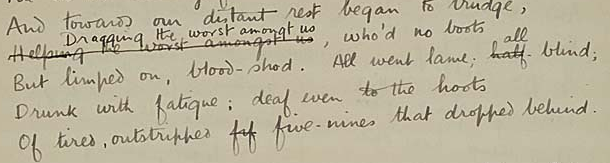
\includegraphics[width=\textwidth]{../Graphics/PHowen.png}                 \par
                     
\bgroup\ttfamily\fontsize{8.5pt}{9pt}\selectfont\par
\begin{exampleblock}{}
\noindent\ttfamily\mbox{}{\color{blue1}<\textbf{l}>}And towards our distant rest began to trudge,{\color{blue1}</\textbf{l}>}\mbox{}\newline 
{\color{blue1}<\textbf{l}>}\mbox{}\newline 
\hspace*{6pt}{\color{blue1}<\textbf{subst}>}\mbox{}\newline 
\hspace*{6pt}\hspace*{6pt}{\color{blue1}<\textbf{del}>}Helping the worst amongst us{\color{blue1}</\textbf{del}>}\mbox{}\newline 
\hspace*{6pt}\hspace*{6pt}{\color{blue1}<\textbf{add}>}Dragging the worst amongt us{\color{blue1}</\textbf{add}>}\mbox{}\newline 
\hspace*{6pt}{\color{blue1}</\textbf{subst}>}, who’d no boots \mbox{}\newline 
{\color{blue1}</\textbf{l}>}\mbox{}\newline 
{\color{blue1}<\textbf{l}>}But limped on, blood-shod. All went lame; {\color{blue1}<\textbf{subst}>}\mbox{}\newline 
\hspace*{6pt}\hspace*{6pt}{\color{blue1}<\textbf{del}>}half-{\color{blue1}</\textbf{del}>}\mbox{}\newline 
\hspace*{6pt}\hspace*{6pt}{\color{blue1}<\textbf{add}>}all{\color{blue1}</\textbf{add}>}\mbox{}\newline 
\hspace*{6pt}{\color{blue1}</\textbf{subst}>} blind;{\color{blue1}</\textbf{l}>}\mbox{}\newline 
{\color{blue1}<\textbf{l}>}Drunk with fatigue ; deaf even to the hoots{\color{blue1}</\textbf{l}>}\mbox{}\newline 
{\color{blue1}<\textbf{l}>}Of tired, outstripped {\color{blue1}<\textbf{del}>}fif{\color{blue1}</\textbf{del}>} five-nines that dropped behind.{\color{blue1}</\textbf{l}>}
\end{exampleblock}
\par\egroup
                       
\end{frame}

\begin{frame}[fragile]
\frametitle{Restitutions de portions de texte dans la transcription}\par
Lorsqu’un mot est restitué par l’éditeur, on peut utiliser l’élément       {\color{blue2}<supplied>}.\par
Il est d’usage de distinguer le texte devenu aujourd’hui illisible ou      disparu par suite de dommages matériels, mais réputé présent à      l’origine dans le document manuscrit (qui est imprimé entre crochets      carrés selon certaines conventions éditoriales), et le texte réputé      omis par inadvertance par le scripteur (imprimé alors le plus souvent      entre crochets pointus). On fera cette distinction dans le fichier TEI      en se servant de l’attribut \emph{@reason} : 
\bgroup\ttfamily\fontsize{8.5pt}{9pt}\selectfont\par
\begin{exampleblock}{}
\noindent\ttfamily\mbox{}{\color{blue1}<\textbf{p}>}…Dragging the worst among{\color{blue1}<\textbf{supplied}\hspace*{6pt}reason="{\color{blue2}omitted}">}s{\color{blue1}</\textbf{supplied}>}t\mbox{}\newline 
 us…{\color{blue1}</\textbf{p}>}
\end{exampleblock}
\par\egroup
       
\end{frame}

\begin{frame}[fragile]
\frametitle{Métadonnées du texte restitué}\par
les attributs \emph{@resp} and \emph{@cert} peuvent être      employés ici comme ailleurs. Un attribut \emph{@source} est      également disponible pour indiquer qu’on se fie à un autre témoin du      texte pour proposer une restitution :     \par
Source de l’exemple : \xref{http://saint-denis.enc.sorbonne.fr/cartulaire.html?chapitre=beaurain&acte=2}{édition critique du cartulaire blanc de Saint-Denis, chapitre de       Beaurain, acte 2}.\par
      
\bgroup\ttfamily\fontsize{8.5pt}{9pt}\selectfont\par
\begin{exampleblock}{}
\noindent\ttfamily\mbox{}{\color{blue1}<\textbf{lem}>}Dampni{\color{blue1}<\textbf{supplied}\hspace*{6pt}source="{\color{blue2}#beaurain-acte2-indiqué-noir}">}pe{\color{blue1}</\textbf{supplied}>}tra{\color{blue1}</\textbf{lem}>}\mbox{}\newline 
{\color{blue1}<\textbf{note}>}\mbox{}\newline 
\hspace*{6pt}{\color{blue1}<\textbf{q}>}pe{\color{blue1}</\textbf{q}>} largement effacé dans B, rétabli d’après l’Anc. inv.\mbox{}\newline 
 noir\mbox{}\newline 
{\color{blue1}</\textbf{note}>}
\end{exampleblock}
\par\egroup
       
\end{frame}

\begin{frame}[fragile]
\frametitle{L’élément {\color{blue2}<gap>}}\par
Lorsque le texte manquant ne peut être rétabli, l’élément à utiliser      est {\color{blue2}<gap>}. à l’aide de l’attribut \emph{@reason}, on pourra      donner la raison de cette lacune dans la transcription, et les      attributs \emph{@extent} et \emph{@unit}donneront la taille      présumée du segment manquant. 
\bgroup\ttfamily\fontsize{8.5pt}{9pt}\selectfont\par
\begin{exampleblock}{}
\noindent\ttfamily\mbox{}{\color{blue1}<\textbf{gap}\hspace*{6pt}reason="{\color{blue2}damage}"\hspace*{6pt}extent="{\color{blue2}7}"\hspace*{6pt}unit="{\color{blue2}chars}"/>}
\end{exampleblock}
\par\egroup
  
\end{frame}

\begin{frame}[fragile]
\frametitle{Autres utilisations de l’élément {\color{blue2}<gap>}}\par
L’élément {\color{blue2}<gap>} peut aussi être utilisé lorsque le segment de      texte, bien présent et lisible, est omis dans la transcription, que ce      soit pour des raisons éditoriales ou parce qu’on a sélectionné les      sections de texte à transcrire. 
\bgroup\ttfamily\fontsize{8.5pt}{9pt}\selectfont\par
\begin{exampleblock}{}
\noindent\ttfamily\mbox{}{\color{blue1}<\textbf{div}\hspace*{6pt}rend="{\color{blue2}slide}">}\mbox{}\newline 
\hspace*{6pt}{\color{blue1}<\textbf{head}>}Lectio x.{\color{blue1}</\textbf{head}>}\mbox{}\newline 
\hspace*{6pt}{\color{blue1}<\textbf{p}>} Hic itaque paterfamilias ad excolendam {\color{blue1}<\textbf{gap}\hspace*{6pt}extent="{\color{blue2}20}"\hspace*{6pt}unit="{\color{blue2}words}"\hspace*{6pt}reason="{\color{blue2}not transcribed}"\hspace*{6pt}resp="{\color{blue2}#DC}"/>} congregare\mbox{}\newline 
\hspace*{6pt}\hspace*{6pt} non desistit. {\color{blue1}</\textbf{p}>}\mbox{}\newline 
{\color{blue1}</\textbf{div}>}
\end{exampleblock}
\par\egroup
       
\end{frame}

\begin{frame}[fragile]
\frametitle{{\color{blue2}<handShift>}}\par
      {\color{blue2}<handShift>} (reprise de main) marque le début d’une section du      texte écrite par une nouvelle main ou le début d’une nouvelle séance      d’écriture.
\bgroup\ttfamily\fontsize{8.5pt}{9pt}\selectfont\par
\begin{exampleblock}{}
\noindent\ttfamily\mbox{}{\color{blue1}<\textbf{l}>}When wolde the cat dwelle in his ynne{\color{blue1}</\textbf{l}>}\mbox{}\newline 
{\color{blue1}<\textbf{handShift}\hspace*{6pt}medium="{\color{blue2}greenish-ink}"/>}\mbox{}\newline 
{\color{blue1}<\textbf{l}>}And if the cattes skynne be slyk {\color{blue1}<\textbf{handShift}\hspace*{6pt}medium="{\color{blue2}black-ink}"/>}\mbox{}\newline 
 and gaye{\color{blue1}</\textbf{l}>}
\end{exampleblock}
\par\egroup
  
\bgroup\ttfamily\fontsize{8.5pt}{9pt}\selectfont\par
\begin{exampleblock}{}
\noindent\ttfamily\mbox{}{\color{blue1}<\textbf{handShift}\hspace*{6pt}new="{\color{blue2}#h1}"\hspace*{6pt}resp="{\color{blue2}#das}"/>}\mbox{}\newline 
{\color{blue1}<\textbf{p}>}... and that good Order Decency and regular worship may be once\mbox{}\newline 
 more introduced and Established in this Parish according to the\mbox{}\newline 
 Rules and Ceremonies of the Church of England and as under a good\mbox{}\newline 
 Consciencious and sober Curate there would and ought to be\mbox{}\newline 
{\color{blue1}<\textbf{handShift}\hspace*{6pt}new="{\color{blue2}#h2}"\hspace*{6pt}resp="{\color{blue2}#das}"/>} and for that purpose the\mbox{}\newline 
 parishioners pray {\color{blue1}</\textbf{p}>}
\end{exampleblock}
\par\egroup
  
\end{frame}

\begin{frame}[fragile]
\frametitle{definition des mains}
\bgroup\ttfamily\fontsize{8.5pt}{9pt}\selectfont\par
\begin{exampleblock}{}
\noindent\ttfamily\mbox{}{\color{blue1}<\textbf{handNotes}>}\mbox{}\newline 
\hspace*{6pt}{\color{blue1}<\textbf{handNote}\hspace*{6pt}xml:id="{\color{blue2}h1}"\hspace*{6pt}script="{\color{blue2}copperplate}">}Carefully written with\mbox{}\newline 
\hspace*{6pt}\hspace*{6pt} regular descenders{\color{blue1}</\textbf{handNote}>}\mbox{}\newline 
\hspace*{6pt}{\color{blue1}<\textbf{handNote}\hspace*{6pt}xml:id="{\color{blue2}h2}"\hspace*{6pt}medium="{\color{blue2}pencil}">}Unschooled scrawl{\color{blue1}</\textbf{handNote}>}\mbox{}\newline 
{\color{blue1}</\textbf{handNotes}>}
\end{exampleblock}
\par\egroup
  
\end{frame}

\begin{frame}[fragile]
\frametitle{Annulation des suppressions}\par
 L’élément {\color{blue2}<restore>} indique une intervention qui conduit au      retour du texte à un état antérieur, par annulation d’une opération ou      instruction de l’éditeur ou de l’auteur. \par
 Si dans la ligne ‘For I hate this my body’ du poème de D. H.      Lawrence \textit{Eloi, Eloi, Lama Sabachthani?}, le mot       ‘my’ a d’abord été supprimé puis restauré en écrivant       ‘stet’ dans la marge, on pourra encoder ce processus ainsi :       
\bgroup\ttfamily\fontsize{8.5pt}{9pt}\selectfont\par
\begin{exampleblock}{}
\noindent\ttfamily\mbox{}{\color{blue1}<\textbf{p}>}[...] For I hate this {\color{blue1}<\textbf{restore}\hspace*{6pt}hand="{\color{blue2}#dhl}"\hspace*{6pt}type="{\color{blue2}marginalStetNote}">}\mbox{}\newline 
\hspace*{6pt}\hspace*{6pt}{\color{blue1}<\textbf{del}>}my{\color{blue1}</\textbf{del}>}\mbox{}\newline 
\hspace*{6pt}{\color{blue1}</\textbf{restore}>} body [...]{\color{blue1}</\textbf{p}>}
\end{exampleblock}
\par\egroup
  \par\begin{exampleblock}{}
... mais cela ne suffit pas pour l'édition génétique\end{exampleblock}\par

\end{frame}

\begin{frame}
\frametitle{L'édition génétique}\par
Un travail en cours, mais avec des résultats déjà apparents.\begin{itemize}

\item quelques éléments supplémentaires pour les transcriptions {\color{blue2}<mod>}, {\color{blue2}<modSpan>}, {\color{blue2}<metaMark>}, {\color{blue2}<used>}, {\color{blue2}<undo>}, {\color{blue2}<redo>}, {\color{blue2}<rewrite>}, {\color{blue2}<transposeGrp>}, {\color{blue2}<transpose>}
\item des mécanismes pour encoder les \emph{étapes d'écriture}, par exemple un attribut \emph{@stage} qui associe n'importe quel élément de la transcription avec une étape identifiée dans l'évolution du document
\item une structuration parallèle du document vu comme object physique, composé des surfaces, zones, et lignes 
\end{itemize} \par\begin{exampleblock}{}
http://www.tei-c.org/Activities/Council/Working/tcw19.html ... à commenter!\end{exampleblock}\par

\end{frame}

\begin{frame}
\frametitle{L'édition en fac-similé }\begin{itemize}

\item Une édition numérique peut etre composée uniquement de pages images, associée avec des metadonnées.  
\item  On peut également identifier des \emph{zones d'interet} dans les images 
\item  Et encoder des liens entre ceux-ci et les parties d'une transcription 
\end{itemize} 
\end{frame}

\begin{frame}[fragile]
\frametitle{ Une solution tres simple}
\bgroup\ttfamily\fontsize{8.5pt}{9pt}\selectfont\par
\begin{exampleblock}{}
\noindent\ttfamily\mbox{}{\color{blue1}<\textbf{TEI}>}\mbox{}\newline 
\hspace*{6pt}{\color{blue1}<\textbf{teiHeader}>}\mbox{}\newline 
\textit{<!--...-->}\mbox{}\newline 
\hspace*{6pt}{\color{blue1}</\textbf{teiHeader}>}\mbox{}\newline 
\hspace*{6pt}{\color{blue1}<\textbf{text}>}\mbox{}\newline 
\hspace*{6pt}\hspace*{6pt}{\color{blue1}<\textbf{pb}\hspace*{6pt}facs="{\color{blue2}page1.png}"/>}\mbox{}\newline 
\textit{<!-- text contained on page 1 may be transcribed here -->}\mbox{}\newline 
\hspace*{6pt}\hspace*{6pt}{\color{blue1}<\textbf{pb}\hspace*{6pt}facs="{\color{blue2}page2.png}"/>}\mbox{}\newline 
\textit{<!-- text contained on page 2 may be transcribed here -->}\mbox{}\newline 
\hspace*{6pt}{\color{blue1}</\textbf{text}>}\mbox{}\newline 
{\color{blue1}</\textbf{TEI}>}
\end{exampleblock}
\par\egroup
  \par
Inconvenients de la solution simplissime... \begin{itemize}

\item doesnt scale well if more complex linking is needed 
\item complicates and obscures digital image info 
\item requires something else (typically mets) 
\end{itemize} 
\end{frame}

\begin{frame}[fragile]
\frametitle{Une solution meilleure }\par
Rassemblement des donnees 
\bgroup\ttfamily\fontsize{8.5pt}{9pt}\selectfont\par
\begin{exampleblock}{}
\noindent\ttfamily\mbox{}{\color{blue1}<\textbf{facsimile}\mbox{}\newline 
\hspace*{6pt}\hspace*{6pt}xml:base="{\color{blue2}http://mylibrary.wibble.fr/blah/blah/blah}">}\mbox{}\newline 
\hspace*{6pt}{\color{blue1}<\textbf{graphic}\hspace*{6pt}url="{\color{blue2}page1.png}"/>}\mbox{}\newline 
\hspace*{6pt}{\color{blue1}<\textbf{graphic}\hspace*{6pt}url="{\color{blue2}page2.png}"/>}\mbox{}\newline 
\hspace*{6pt}{\color{blue1}<\textbf{graphic}\hspace*{6pt}url="{\color{blue2}page3.png}"/>}\mbox{}\newline 
\hspace*{6pt}{\color{blue1}<\textbf{graphic}\hspace*{6pt}url="{\color{blue2}page4.png}"/>}\mbox{}\newline 
{\color{blue1}</\textbf{facsimile}>}
\end{exampleblock}
\par\egroup
  
\end{frame}

\begin{frame}[fragile]
\frametitle{Maintenant, si on a des versions alternatives?}\par
On se sert de {\color{blue2}<surface>} pour regrouper les images équivalentes: 
\bgroup\ttfamily\fontsize{8.5pt}{9pt}\selectfont\par
\begin{exampleblock}{}
\noindent\ttfamily\mbox{}{\color{blue1}<\textbf{facsimile}>}\mbox{}\newline 
\hspace*{6pt}{\color{blue1}<\textbf{graphic}\hspace*{6pt}url="{\color{blue2}page1.png}"/>}\mbox{}\newline 
\hspace*{6pt}{\color{blue1}<\textbf{surface}>}\mbox{}\newline 
\hspace*{6pt}\hspace*{6pt}{\color{blue1}<\textbf{graphic}\hspace*{6pt}url="{\color{blue2}page2-highRes.png}"/>}\mbox{}\newline 
\hspace*{6pt}\hspace*{6pt}{\color{blue1}<\textbf{graphic}\hspace*{6pt}url="{\color{blue2}page2-lowRes.png}"/>}\mbox{}\newline 
\hspace*{6pt}{\color{blue1}</\textbf{surface}>}\mbox{}\newline 
\hspace*{6pt}{\color{blue1}<\textbf{graphic}\hspace*{6pt}url="{\color{blue2}page3.png}"/>}\mbox{}\newline 
\hspace*{6pt}{\color{blue1}<\textbf{graphic}\hspace*{6pt}url="{\color{blue2}page4.png}"/>}\mbox{}\newline 
{\color{blue1}</\textbf{facsimile}>}
\end{exampleblock}
\par\egroup
  
\end{frame}

\begin{frame}[fragile]
\frametitle{Liaison image/ transcription}
\bgroup\ttfamily\fontsize{8.5pt}{9pt}\selectfont\par
\begin{exampleblock}{}
\noindent\ttfamily\mbox{}{\color{blue1}<\textbf{facsimile}>}\mbox{}\newline 
\hspace*{6pt}{\color{blue1}<\textbf{graphic}\hspace*{6pt}xml:id="{\color{blue2}page1}"\hspace*{6pt}url="{\color{blue2}page1.png}"/>}\mbox{}\newline 
\hspace*{6pt}{\color{blue1}<\textbf{graphic}\hspace*{6pt}xml:id="{\color{blue2}page2}"\hspace*{6pt}url="{\color{blue2}page2.png}"/>}\mbox{}\newline 
\hspace*{6pt}{\color{blue1}<\textbf{graphic}\hspace*{6pt}xml:id="{\color{blue2}page3}"\hspace*{6pt}url="{\color{blue2}page3.png}"/>}\mbox{}\newline 
\hspace*{6pt}{\color{blue1}<\textbf{graphic}\hspace*{6pt}xml:id="{\color{blue2}page4}"\hspace*{6pt}url="{\color{blue2}page4.png}"/>}\mbox{}\newline 
{\color{blue1}</\textbf{facsimile}>}\mbox{}\newline 
\textit{<!-- ... -->}\mbox{}\newline 
{\color{blue1}<\textbf{text}>}\mbox{}\newline 
\hspace*{6pt}{\color{blue1}<\textbf{pb}\hspace*{6pt}facs="{\color{blue2}#page1}"/>}\mbox{}\newline 
\textit{<!-- text contained on page 1 may be encoded here -->}\mbox{}\newline 
\hspace*{6pt}{\color{blue1}<\textbf{pb}\hspace*{6pt}facs="{\color{blue2}#page2}"/>}\mbox{}\newline 
\textit{<!-- text contained on page 2 may be encoded here -->}\mbox{}\newline 
{\color{blue1}</\textbf{text}>}
\end{exampleblock}
\par\egroup
  
\end{frame}

\begin{frame}
\frametitle{ Cette methode est tres generale}\begin{itemize}

\item {\color{blue2}<surface>} definit une système de co-ordinés 
\item {\color{blue2}<zone>} definit un zone d'interet 
\item des {\color{blue2}<graphic>}s sont disponible a n'importe quel niveau 
\end{itemize} 
\end{frame}

\begin{frame}
\frametitle{ Bovelles-49r.png}\par
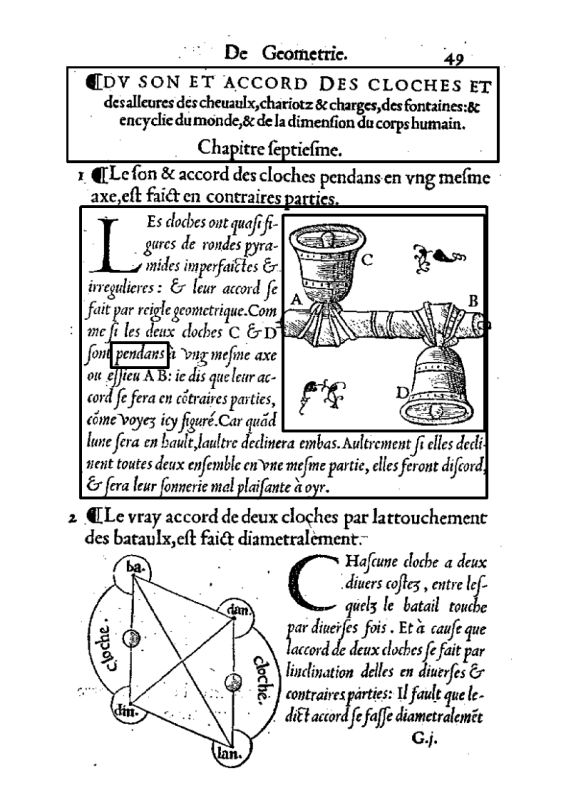
\includegraphics[height=300pt,]{../Graphics/facs-fig1.png}
\end{frame}

\begin{frame}[fragile]
\frametitle{ Encodage du fac-similé}
\bgroup\ttfamily\fontsize{6.5pt}{7pt}\selectfont\par
\begin{exampleblock}{}
\noindent\ttfamily\mbox{}{\color{blue1}<\textbf{facsimile}>}\mbox{}\newline 
\hspace*{6pt}{\color{blue1}<\textbf{surface}\hspace*{6pt}ulx="{\color{blue2}0}"\hspace*{6pt}uly="{\color{blue2}0}"\hspace*{6pt}lrx="{\color{blue2}200}"\hspace*{6pt}lry="{\color{blue2}300}">}\mbox{}\newline 
\hspace*{6pt}\hspace*{6pt}{\color{blue1}<\textbf{zone}\hspace*{6pt}xml:id="{\color{blue2}B49r}"\hspace*{6pt}ulx="{\color{blue2}0}"\hspace*{6pt}uly="{\color{blue2}0}"\hspace*{6pt}lrx="{\color{blue2}200}"\hspace*{6pt}lry="{\color{blue2}300}">}\mbox{}\newline 
\hspace*{6pt}\hspace*{6pt}\hspace*{6pt}{\color{blue1}<\textbf{graphic}\hspace*{6pt}url="{\color{blue2}Bovelles-49r.png}"/>}\mbox{}\newline 
\hspace*{6pt}\hspace*{6pt}{\color{blue1}</\textbf{zone}>}\mbox{}\newline 
\hspace*{6pt}\hspace*{6pt}{\color{blue1}<\textbf{zone}\hspace*{6pt}ulx="{\color{blue2}105}"\hspace*{6pt}uly="{\color{blue2}76}"\hspace*{6pt}lrx="{\color{blue2}175}"\hspace*{6pt}lry="{\color{blue2}160}">}\mbox{}\newline 
\hspace*{6pt}\hspace*{6pt}\hspace*{6pt}{\color{blue1}<\textbf{graphic}\hspace*{6pt}url="{\color{blue2}Bovelles49r-detail.png}"/>}\mbox{}\newline 
\hspace*{6pt}\hspace*{6pt}{\color{blue1}</\textbf{zone}>}\mbox{}\newline 
\hspace*{6pt}\hspace*{6pt}{\color{blue1}<\textbf{zone}\hspace*{6pt}xml:id="{\color{blue2}B49rHead}"\hspace*{6pt}ulx="{\color{blue2}25}"\hspace*{6pt}uly="{\color{blue2}25}"\hspace*{6pt}lrx="{\color{blue2}180}"\hspace*{6pt}lry="{\color{blue2}60}"/>}\mbox{}\newline 
\textit{<!-- contains the title -->}\mbox{}\newline 
\hspace*{6pt}\hspace*{6pt}{\color{blue1}<\textbf{zone}\hspace*{6pt}xml:id="{\color{blue2}B49rPara2}"\hspace*{6pt}ulx="{\color{blue2}28}"\hspace*{6pt}uly="{\color{blue2}75}"\hspace*{6pt}lrx="{\color{blue2}175}"\hspace*{6pt}lry="{\color{blue2}178}"/>}\mbox{}\newline 
\textit{<!-- contains the paragraph in italics -->}\mbox{}\newline 
\hspace*{6pt}\hspace*{6pt}{\color{blue1}<\textbf{zone}\hspace*{6pt}xml:id="{\color{blue2}B49rFig1}"\hspace*{6pt}ulx="{\color{blue2}105}"\hspace*{6pt}uly="{\color{blue2}76}"\hspace*{6pt}lrx="{\color{blue2}175}"\hspace*{6pt}lry="{\color{blue2}160}"/>}\mbox{}\newline 
\textit{<!-- contains the figure -->}\mbox{}\newline 
\hspace*{6pt}\hspace*{6pt}{\color{blue1}<\textbf{zone}\hspace*{6pt}xml:id="{\color{blue2}B49rW457}"\hspace*{6pt}ulx="{\color{blue2}45}"\hspace*{6pt}uly="{\color{blue2}125}"\hspace*{6pt}lrx="{\color{blue2}60}"\hspace*{6pt}lry="{\color{blue2}130}"/>}\mbox{}\newline 
\textit{<!-- contains the word "pendans" -->}\mbox{}\newline 
\hspace*{6pt}{\color{blue1}</\textbf{surface}>}\mbox{}\newline 
{\color{blue1}</\textbf{facsimile}>}
\end{exampleblock}
\par\egroup
  \par
(Nota: on a proposé des identifiants pour chaque zone)
\end{frame}

\begin{frame}[fragile]
\frametitle{Encodage de la transcription}
\bgroup\ttfamily\fontsize{6.5pt}{7pt}\selectfont\par
\begin{exampleblock}{}
\noindent\ttfamily\mbox{}{\color{blue1}<\textbf{pb}\hspace*{6pt}facs="{\color{blue2}#B49r}"/>}\mbox{}\newline 
{\color{blue1}<\textbf{fw}>}De Geometrie 49{\color{blue1}</\textbf{fw}>}\mbox{}\newline 
{\color{blue1}<\textbf{head}\hspace*{6pt}facs="{\color{blue2}#B49rHead}">}DU SON ET ACCORD DES CLOCHES ET {\color{blue1}<\textbf{lb}/>} des alleures des chevaulx,\mbox{}\newline 
 chariotz & charges, des fontaines:& {\color{blue1}<\textbf{lb}/>} encyclie du monde,\mbox{}\newline 
 & de la dimension du corps humain.{\color{blue1}</\textbf{head}>}\mbox{}\newline 
{\color{blue1}<\textbf{head}>}Chapitre septiesme{\color{blue1}</\textbf{head}>}\mbox{}\newline 
{\color{blue1}<\textbf{div}\hspace*{6pt}n="{\color{blue2}1}">}\mbox{}\newline 
\hspace*{6pt}{\color{blue1}<\textbf{p}>}Le son & accord des cloches pendans en ung mesme {\color{blue1}<\textbf{lb}/>} axe, est\mbox{}\newline 
\hspace*{6pt}\hspace*{6pt} faict en contraires parties.{\color{blue1}</\textbf{p}>}\mbox{}\newline 
\hspace*{6pt}{\color{blue1}<\textbf{p}\hspace*{6pt}rend="{\color{blue2}it}"\hspace*{6pt}facs="{\color{blue2}#B49rPara2}">}LEs cloches ont quasi fi{\color{blue1}<\textbf{lb}/>}gures de rondes\mbox{}\newline 
\hspace*{6pt}\hspace*{6pt} pyra{\color{blue1}<\textbf{lb}/>}mides imperfaictes & {\color{blue1}<\textbf{lb}/>} irregulieres: & leur\mbox{}\newline 
\hspace*{6pt}\hspace*{6pt} accord se {\color{blue1}<\textbf{lb}/>} fait par reigle geometrique. Com{\color{blue1}<\textbf{lb}/>}me si les deux\mbox{}\newline 
\hspace*{6pt}\hspace*{6pt} cloches C & D {\color{blue1}<\textbf{lb}/>} sont {\color{blue1}<\textbf{w}\hspace*{6pt}facs="{\color{blue2}#B49rW457}">}pendans{\color{blue1}</\textbf{w}>} à ung\mbox{}\newline 
\hspace*{6pt}\hspace*{6pt} mesme axe {\color{blue1}<\textbf{lb}/>} ou essieu A B: je dis que leur ac{\color{blue1}<\textbf{lb}/>}cord se fera en\mbox{}\newline 
\hspace*{6pt}\hspace*{6pt} co{\color{blue1}<\textbf{ex}>}n{\color{blue1}</\textbf{ex}>}traires parties{\color{blue1}<\textbf{lb}/>} co{\color{blue1}<\textbf{ex}>}m{\color{blue1}</\textbf{ex}>}me voyez icy\mbox{}\newline 
\hspace*{6pt}\hspace*{6pt} figuré. Car qua{\color{blue1}<\textbf{ex}>}n{\color{blue1}</\textbf{ex}>}d {\color{blue1}<\textbf{lb}/>} lune sera en hault, laultre\mbox{}\newline 
\hspace*{6pt}\hspace*{6pt} declinera embas. Aultrement si elles decli{\color{blue1}<\textbf{lb}/>}nent toutes deux\mbox{}\newline 
\hspace*{6pt}\hspace*{6pt} ensembles en une mesme partie, elles seront discord, {\color{blue1}<\textbf{lb}/>} & sera\mbox{}\newline 
\hspace*{6pt}\hspace*{6pt} leur sonnerie mal plaisante à oyr.{\color{blue1}<\textbf{figure}\hspace*{6pt}facs="{\color{blue2}#B49rFig1}"/>}\mbox{}\newline 
\hspace*{6pt}{\color{blue1}</\textbf{p}>}\mbox{}\newline 
{\color{blue1}</\textbf{div}>}
\end{exampleblock}
\par\egroup
  
\end{frame}

\begin{frame}
\frametitle{Travaux pratiques}
    \noindent
  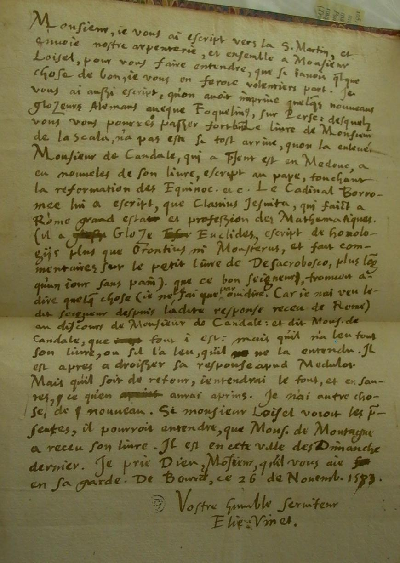
\includegraphics[width=\textwidth]{../Graphics/vinet.png}
\end{frame}

\begin{frame}
\frametitle{Travaux pratiques}\par
Enrichissez la transcription qui se trouve dans \textsf{vinet.txt}\par
 \begin{itemize}

\item balisage des ratures avec {\color{blue2}<del>}
\item balisage des abbréviations avec {\color{blue2}<choice>}, {\color{blue2}<abbr>}, {\color{blue2}<expan>}, ou bien {\color{blue2}<am>} et {\color{blue2}<ex>}
\end{itemize}  
\end{frame}

\end{document}
